% THIS DOCUMENT IS TAILORED TO REQUIREMENTS FOR SCIENTIFIC COMPUTING.  IT SHOULDN'T
% BE USED FOR NON-SCIENTIFIC COMPUTING PROJECTS
\documentclass[12pt]{article}

\usepackage{amsmath, mathtools}
\usepackage{amsfonts}
\usepackage{amssymb}
\usepackage{graphicx}
\usepackage{colortbl}
\usepackage{xr}
\usepackage{hyperref}
\usepackage{longtable}
\usepackage{xfrac}
\usepackage{tabularx}
\usepackage{float}
\usepackage{siunitx}
\usepackage{booktabs}
\usepackage{caption}
\usepackage{pdflscape}
\usepackage{afterpage}

\usepackage[round]{natbib}

\usepackage{hyperref}
%\usepackage{refcheck}

\hypersetup{
    bookmarks=true,         % show bookmarks bar?
      colorlinks=true,       % false: boxed links; true: colored links
    linkcolor=red,          % color of internal links (change box color with linkbordercolor)
    citecolor=green,        % color of links to bibliography
    filecolor=magenta,      % color of file links
    urlcolor=cyan           % color of external links
}

%% Comments

\usepackage{color}

\newif\ifcomments\commentstrue %displays comments
%\newif\ifcomments\commentsfalse %so that comments do not display

\ifcomments
\newcommand{\authornote}[3]{\textcolor{#1}{[#3 ---#2]}}
\newcommand{\todo}[1]{\textcolor{red}{[TODO: #1]}}
\else
\newcommand{\authornote}[3]{}
\newcommand{\todo}[1]{}
\fi

\newcommand{\wss}[1]{\authornote{blue}{SS}{#1}} 
\newcommand{\plt}[1]{\authornote{magenta}{TPLT}{#1}} %For explanation of the template
\newcommand{\an}[1]{\authornote{cyan}{Author}{#1}}

%% Common Parts

\newcommand{\progname}{ProgName} % PUT YOUR PROGRAM NAME HERE
\newcommand{\authname}{Team \#, Team Name
\\ Student 1 name
\\ Student 2 name
\\ Student 3 name
\\ Student 4 name} % AUTHOR NAMES                  

\usepackage{hyperref}
    \hypersetup{colorlinks=true, linkcolor=blue, citecolor=blue, filecolor=blue,
                urlcolor=blue, unicode=false}
    \urlstyle{same}
                                


% For easy change of table widths
\newcommand{\colZwidth}{1.0\textwidth}
\newcommand{\colAwidth}{0.13\textwidth}
\newcommand{\colBwidth}{0.82\textwidth}
\newcommand{\colCwidth}{0.1\textwidth}
\newcommand{\colDwidth}{0.05\textwidth}
\newcommand{\colEwidth}{0.8\textwidth}
\newcommand{\colFwidth}{0.17\textwidth}
\newcommand{\colGwidth}{0.5\textwidth}
\newcommand{\colHwidth}{0.28\textwidth}

% Used so that cross-references have a meaningful prefix
\newcounter{defnum} %Definition Number
\newcommand{\dthedefnum}{GD\thedefnum}
\newcommand{\dref}[1]{GD\ref{#1}}
\newcounter{datadefnum} %Datadefinition Number
\newcommand{\ddthedatadefnum}{DD\thedatadefnum}
\newcommand{\ddref}[1]{DD\ref{#1}}
\newcounter{theorynum} %Theory Number
\newcommand{\tthetheorynum}{TM\thetheorynum}
\newcommand{\tref}[1]{TM\ref{#1}}
\newcounter{tablenum} %Table Number
\newcommand{\tbthetablenum}{TB\thetablenum}
\newcommand{\tbref}[1]{TB\ref{#1}}
\newcounter{assumpnum} %Assumption Number
\newcommand{\atheassumpnum}{A\theassumpnum}
\newcommand{\aref}[1]{A\ref{#1}}
\newcounter{goalnum} %Goal Number
\newcommand{\gthegoalnum}{GS\thegoalnum}
\newcommand{\gsref}[1]{GS\ref{#1}}
\newcounter{instnum} %Instance Number
\newcommand{\itheinstnum}{IM\theinstnum}
\newcommand{\iref}[1]{IM\ref{#1}}
\newcounter{reqnum} %Requirement Number
\newcommand{\rthereqnum}{R\thereqnum}
\newcommand{\rref}[1]{R\ref{#1}}
\newcounter{nfrnum} %NFR Number
\newcommand{\rthenfrnum}{NFR\thenfrnum}
\newcommand{\nfrref}[1]{NFR\ref{#1}}
\newcounter{lcnum} %Likely change number
\newcommand{\lthelcnum}{LC\thelcnum}
\newcommand{\lcref}[1]{LC\ref{#1}}

\usepackage{fullpage}

\newcommand{\deftheory}[9][Not Applicable]
{
\newpage
\noindent \rule{\textwidth}{0.5mm}

\paragraph{RefName: } \textbf{#2} \phantomsection 
\label{#2}

\paragraph{Label:} #3

\noindent \rule{\textwidth}{0.5mm}

\paragraph{Equation:}

#4

\paragraph{Description:}

#5

\paragraph{Notes:}

#6

\paragraph{Source:}

#7

\paragraph{Ref.\ By:}

#8

\paragraph{Preconditions for \hyperref[#2]{#2}:}
\label{#2_precond}

#9

\paragraph{Derivation for \hyperref[#2]{#2}:}
\label{#2_deriv}

#1

\noindent \rule{\textwidth}{0.5mm}

}

\DeclareSIUnit{\cellunit}{cu}  % 'cu' is the symbol that will appear



\begin{document}

\title{Software Requirements Specification for \progname} 
\author{Uriel Garcilazo Cruz}
\date{\today}
	
\maketitle

~\newpage

\pagenumbering{roman}

\tableofcontents

~\newpage

\section*{Revision History}

\begin{tabularx}{\textwidth}{p{3cm}p{2cm}X}
\toprule {\bf Date} & {\bf Version} & {\bf Notes}\\
\midrule
February 1 2025 & 1.0 & Document Creation\\
% Date 2 & 1.1 & Notes\\
\bottomrule
\end{tabularx}

% ~\\
% \plt{This template is intended for use by CAS 741.  For CAS 741 the template
% should be used exactly as given, except the Reflection Appendix can be deleted.
% For the capstone course it is a source of ideas, but shouldn't be followed
% exactly.  The exception is the reflection appendix.  All capstone SRS documents
% should have a reflection appendix.}

~\newpage

\section{Reference Material}

This section records information for easy reference.

\subsection{Table of Units}

Throughout this document SI (Syst\`{e}me International d'Unit\'{e}s) is NOT employed
as the unit system.  Instead of the basic units from SI, the standard Human Genome
 Variation Society (HGVS) nomenclature is employed as the unit system, unless 
otherwise noted.


~\newline

\renewcommand{\arraystretch}{1.2}
\begin{center}
  \begin{tabular}{l l l} 
    \toprule		
    \textbf{symbol} & \textbf{unit} & \textbf{HGVS}\\
    \midrule 
    qa & alignment quality & fundamental unit of alignment quality 
    (unit definition is unique to this document)
    \\
    bp & base pair & fundamental unit of genetic sequence length
    \\
    Kb & kilobase unit & one thousand base pairs
    \\
    \bottomrule
  \end{tabular}
\end{center}

~\newline

  %	\caption{Provide a caption}
%\end{table}

% \plt{Only include the units that your SRS actually uses.}

% \plt{Derived units, like newtons, pascal, etc, should show their derivation
%     (the units they are derived from) if their constituent units are in the
%     table of units (that is, if the units they are derived from are used in the
%     document).  For instance, the derivation of pascals as
%     $\si{\pascal}=\si{\newton\per\square\meter}$ is shown if newtons and m are
%     both in the table.  The derivations of newtons would not be shown if kg and
%     s are not both in the table.}

% \plt{The symbol for units named after people use capital letters, but the name
%   of the unit itself uses lower case.  For instance, pascals use the symbol Pa,
%   watts use the symbol W, teslas use the symbol T, newtons use the symbol N,
%   etc.  The one exception to this is degree Celsius.  Details on writing metric
%   units can be found on the 
%   \href{https://www.nist.gov/pml/weights-and-measures/writing-metric-units}
%   {NIST} web-page.}

\subsection{Table of Symbols}

The table that follows summarizes the symbols used in this document along with
their units.  The choice of symbols was made to be consistent with the bioinformatics
literature and with the existing internationally recognized standard for the description
 of DNA, RNA and protein reading frames. The symbols are listed in alphabetical order.

\renewcommand{\arraystretch}{1.2}
%\noindent \begin{tabularx}{1.0\textwidth}{l l X}
\noindent \begin{longtable*}{l l p{12cm}} \toprule
\textbf{symbol} & \textbf{unit} & \textbf{description}\\
\midrule 
  F & -- & Comparative alignment between two sequences
  \\
  g & qa & penalty associated with a gap in the alignment of two sequences
  \\
  $N_A$ & bp & Adenine nitrogenous base, element of the purine family of nucleotides with an amine group in Carbon 6 of its pyrimidine ring
  \\
  $N_C$ & bp & Cytosine nitrogenous base, element of the pyrimidine family of nucleotides with a no methylated carbons making part of its pyrimidine ring
  \\
  $N_G$ & bp & Guanine nitrogenous base, element of the purine family of nucleotides with an amine group on Carbon 2 and a carbonyl group on Carbon 6 of its pyrimidine ring
  \\
  $N_T$ & bp & Tymine nitrogenous base, element of the pyrimidine family of nucleotides with a methyl group in Carbon 5 of its pyrimidine ring
  \\
  $Q_{AB}$ & qa & A collection of base pairs representing a genetic sequence to be compared with another sequence $SEQ_A$
  \\
  S & qa & Substitution matrix used to score the alignment of two sequences
  \\
  $SEQ_A$ & Kb & A collection of base pairs representing a genetic sequence to be compared with another sequence $SEQ_B$
  \\
  $SEQ_B$ & Kb & A collection of base pairs representing a genetic sequence to be compared with another sequence $SEQ_A$
  \\
  SNP & bp & single nucleotide polymorphism; variation in a single base pair in DNA sequence
  \\
  $T_I$ & qa & A transition occurrying between nucleotides of the same nitrogenous base families
  \\
  $T_V$ & qa & A transition occurrying between nucleotides of different nitrogenous base families
  \\
\bottomrule
\end{longtable*}
% \plt{Use your problems actual symbols.  The si package is a good idea to use for
  % units.}

\subsection{Abbreviations and Acronyms}

\renewcommand{\arraystretch}{1.2}
\begin{tabular}{l l} 
  \toprule		
  \textbf{symbol} & \textbf{description}\\
  \midrule 
  HGVS & Human Genome Variation Society\\
  A & Assumption\\
  DD & Data Definition\\
  GD & General Definition\\
  GS & Goal Statement\\
  IM & Instance Model\\
  LC & Likely Change\\
  PS & Physical System Description\\
  R & Requirement\\
  SRS & Software Requirements Specification\\
  \progname{} & Substitution Matrix benchmarking with pairwise alignment\\
  TM & Theoretical Model\\
  \bottomrule
\end{tabular}\\



\section{Introduction}

Substitution matrices are critical assumptions that greatly impact studies
in the area of comparative biology, yet, benchmarking these matrices is a 
laborious task.

The following section contains an overview of the Software Requirements Specification (SRS)
for a substitution matrix benchmark tool via pairwise alignment. The program is referred to 
as SubLiMat. The purpose of this section is to characterize the purpose, scope of Requirements, 
characteristics of Intended Reader, and Organization of the SRS document.

% \plt{The introduction section is written to introduce the problem.  It starts
%   general and focuses on the problem domain. The general advice is to start with
% a paragraph or two that describes the problem, followed by a ``roadmap''
% paragraph.  A roadmap orients the reader by telling them what sub-sections to
% expect in the Introduction section.}

\subsection{Purpose of Document}

The purpose of this document is to provide a detailed and standardized characterization of 
the elements, theoretical and operational, that surround the SubLiMat software. Such 
elements include goals, assumptions, and theoretical and instanced models that describe 
the scientific basis of the software. Moreover, the document is intended to be used as a guide to detail 
the unique characteristics of the software to improve on its verifiability and correctness. 


\subsection{Scope of Requirements} 

The scope of the requirements for the SubLiMat software includes the evaluation of 
moderate-sized genetic sequences with similar dimensions. 



% \plt{The scope section is relevant for later determining typical values of inputs. The scope should make it clear what inputs are reasonable to expect. This is a distinction between scope and context (context is a later section).  Scope affects the inputs while context affects how the software will be used.}

\subsection{Characteristics of Intended Reader} \label{sec_IntendedReader}

The intended readers of this documentation should have a general understanding of genetics, 
equivalent or higher to a highschool level. Although not necessary, the document may benefit
from a reader who possesses a basic understanding of comparative biology equivalent to first 
year university level or higher.  



\subsection{Organization of Document}

The structure of this document follows the standard template for an SRS document.
As presented by \href{https://jacquescarette.github.io/Drasil/examples/swhsnopcm/SRS/HTML/SWHSNoPCM_SRS.html}
{Jegatheesan \& Smith, 2019} in their SRS example for this section:

\begin{quote}
The organization of this document follows the template for an SRS for scientific 
computing software proposed by \cite{koothoor2013}, \cite{smithLai2005}, 
\cite{smithEtAl2007}, and \cite{smithKoothoor2016}. The presentation follows 
the standard pattern of presenting goals, theories, definitions, and assumptions.
\dots


The goal statements are refined to the theoretical models and the theoretical 
models to the instance models.
\end{quote}
% \plt{This section provides a roadmap of the SRS document.  It will help the
%   reader orient themselves.  It will provide direction that will help them
%   select which sections they want to read, and in what order.  This section will
%   be similar between project.}

\section{General System Description}

This section provides general information about the system.  It identifies the
interfaces between the system and its environment, describes the user
characteristics and lists the system constraints.

\subsection{System Context}


\begin{figure}[h!]
\begin{center}
 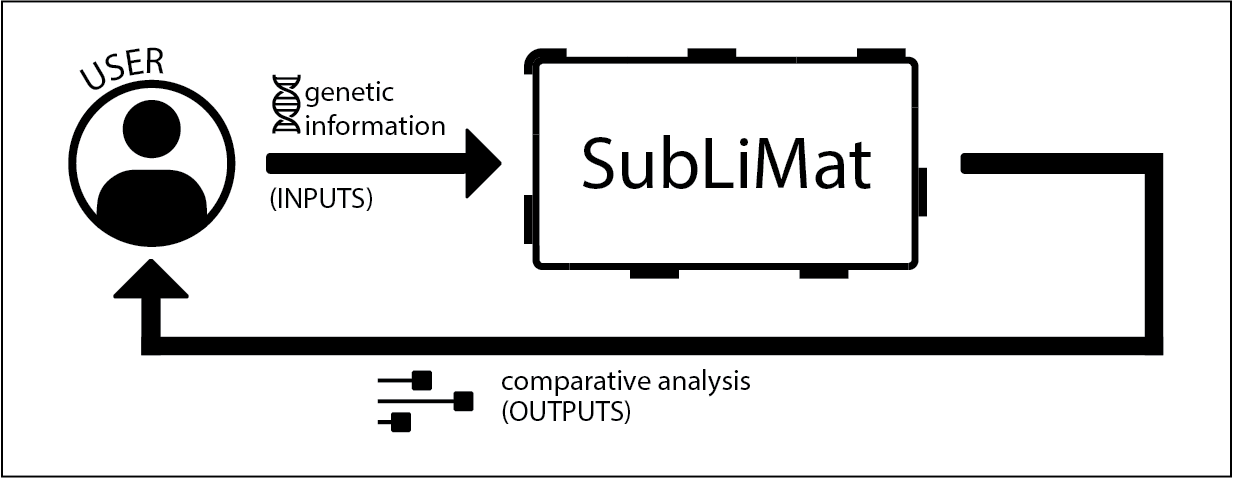
\includegraphics[width=0.8\textwidth]{sublimat_SystemContextFigure}
\caption{System Context}
\label{Fig_SystemContext} 
\end{center}
\end{figure}


\begin{itemize}
\item User Responsibilities:
\begin{itemize}
\item Provide genetic sequences of DNA
\item Provide meaningful genetic sequences presumed to share a common ancestor
\item Provide genetic sequences of similar dimensions
\end{itemize}
\item \progname{} Responsibilities:
\begin{itemize}
\item Detect data type mismatch, such as a string of characters instead of a
  floating point number
\item Determine if there exist any base pairs in the genetic sequences that are
  not part of the standard genetic code nomenclature for DNA
\item Calculate the alignment quality between two genetic sequences to produce outputs
\end{itemize}
\end{itemize}



\subsection{User Characteristics} \label{SecUserCharacteristics}

The end user of SubLiMat should have a general understanding of genetics and be familiar 
with the use of genetic sequences to make hypotheses of common ancestry.


\subsection{System Constraints}

No contraints were integrated in the program design that weren't at the scope of the 
\progname{} software's operational implementation.


\section{Specific System Description}




\subsection{Problem Description} \label{Sec_pd}

\progname{} is intended to solve the uncertainties associated with the influence of 
substitution matrices on the alignment quality of genetic sequences.
% ... \plt{What problem does your program solve?
% The description here should be in the problem space, not the solution space.}

\subsubsection{Terminology and  Definitions}



This subsection provides a list of terms that are used in the subsequent
sections and their meaning, with the purpose of reducing ambiguity and making it
easier to correctly understand the requirements:

\begin{itemize}

\item Substitution matrix: A square matrix that summarizes 
the rewards or penalties of moving from one base pair to another and 
expressed in units of alignment quality (qa)
\item Pairwise alignment: A pairwise alignment is the process of aligning two genetic 
sequences to identify regions of similarity 
\item Genetic sequence: A genetic sequence is a string of characters $\in \{N_A, N_C, N_G, N_T\}$ that represent 
the nucleotides of a DNA molecule and expressed in units of base pairs (bp)
\item Alignment quality: A measure of the quality of the alignment between two genetic 
sequences and express in units of alignment quality (qa)
\item gap: A gap is a space in the alignment of two genetic sequences that represents
a deletion or insertion of a base pair, and penalized with units of alignment quality (qa)

\end{itemize}

\subsubsection{Physical System Description} \label{sec_phySystDescrip}


The physical system of \progname{}, as shown in Figure~\ref{fig:sequence_alignment},
includes the following elements:

\begin{itemize}

\item[PS1:] sequence $SEQ_A$ and sequence $SEQ_B$

\item[PS2:] Pairwise comparison matrix $F$ between the two sequences

\end{itemize}

% \plt{A figure here makes sense for most SRS documents}
\begin{figure}[h!]
  \begin{center}
  %\rotatebox{-90}
  {
   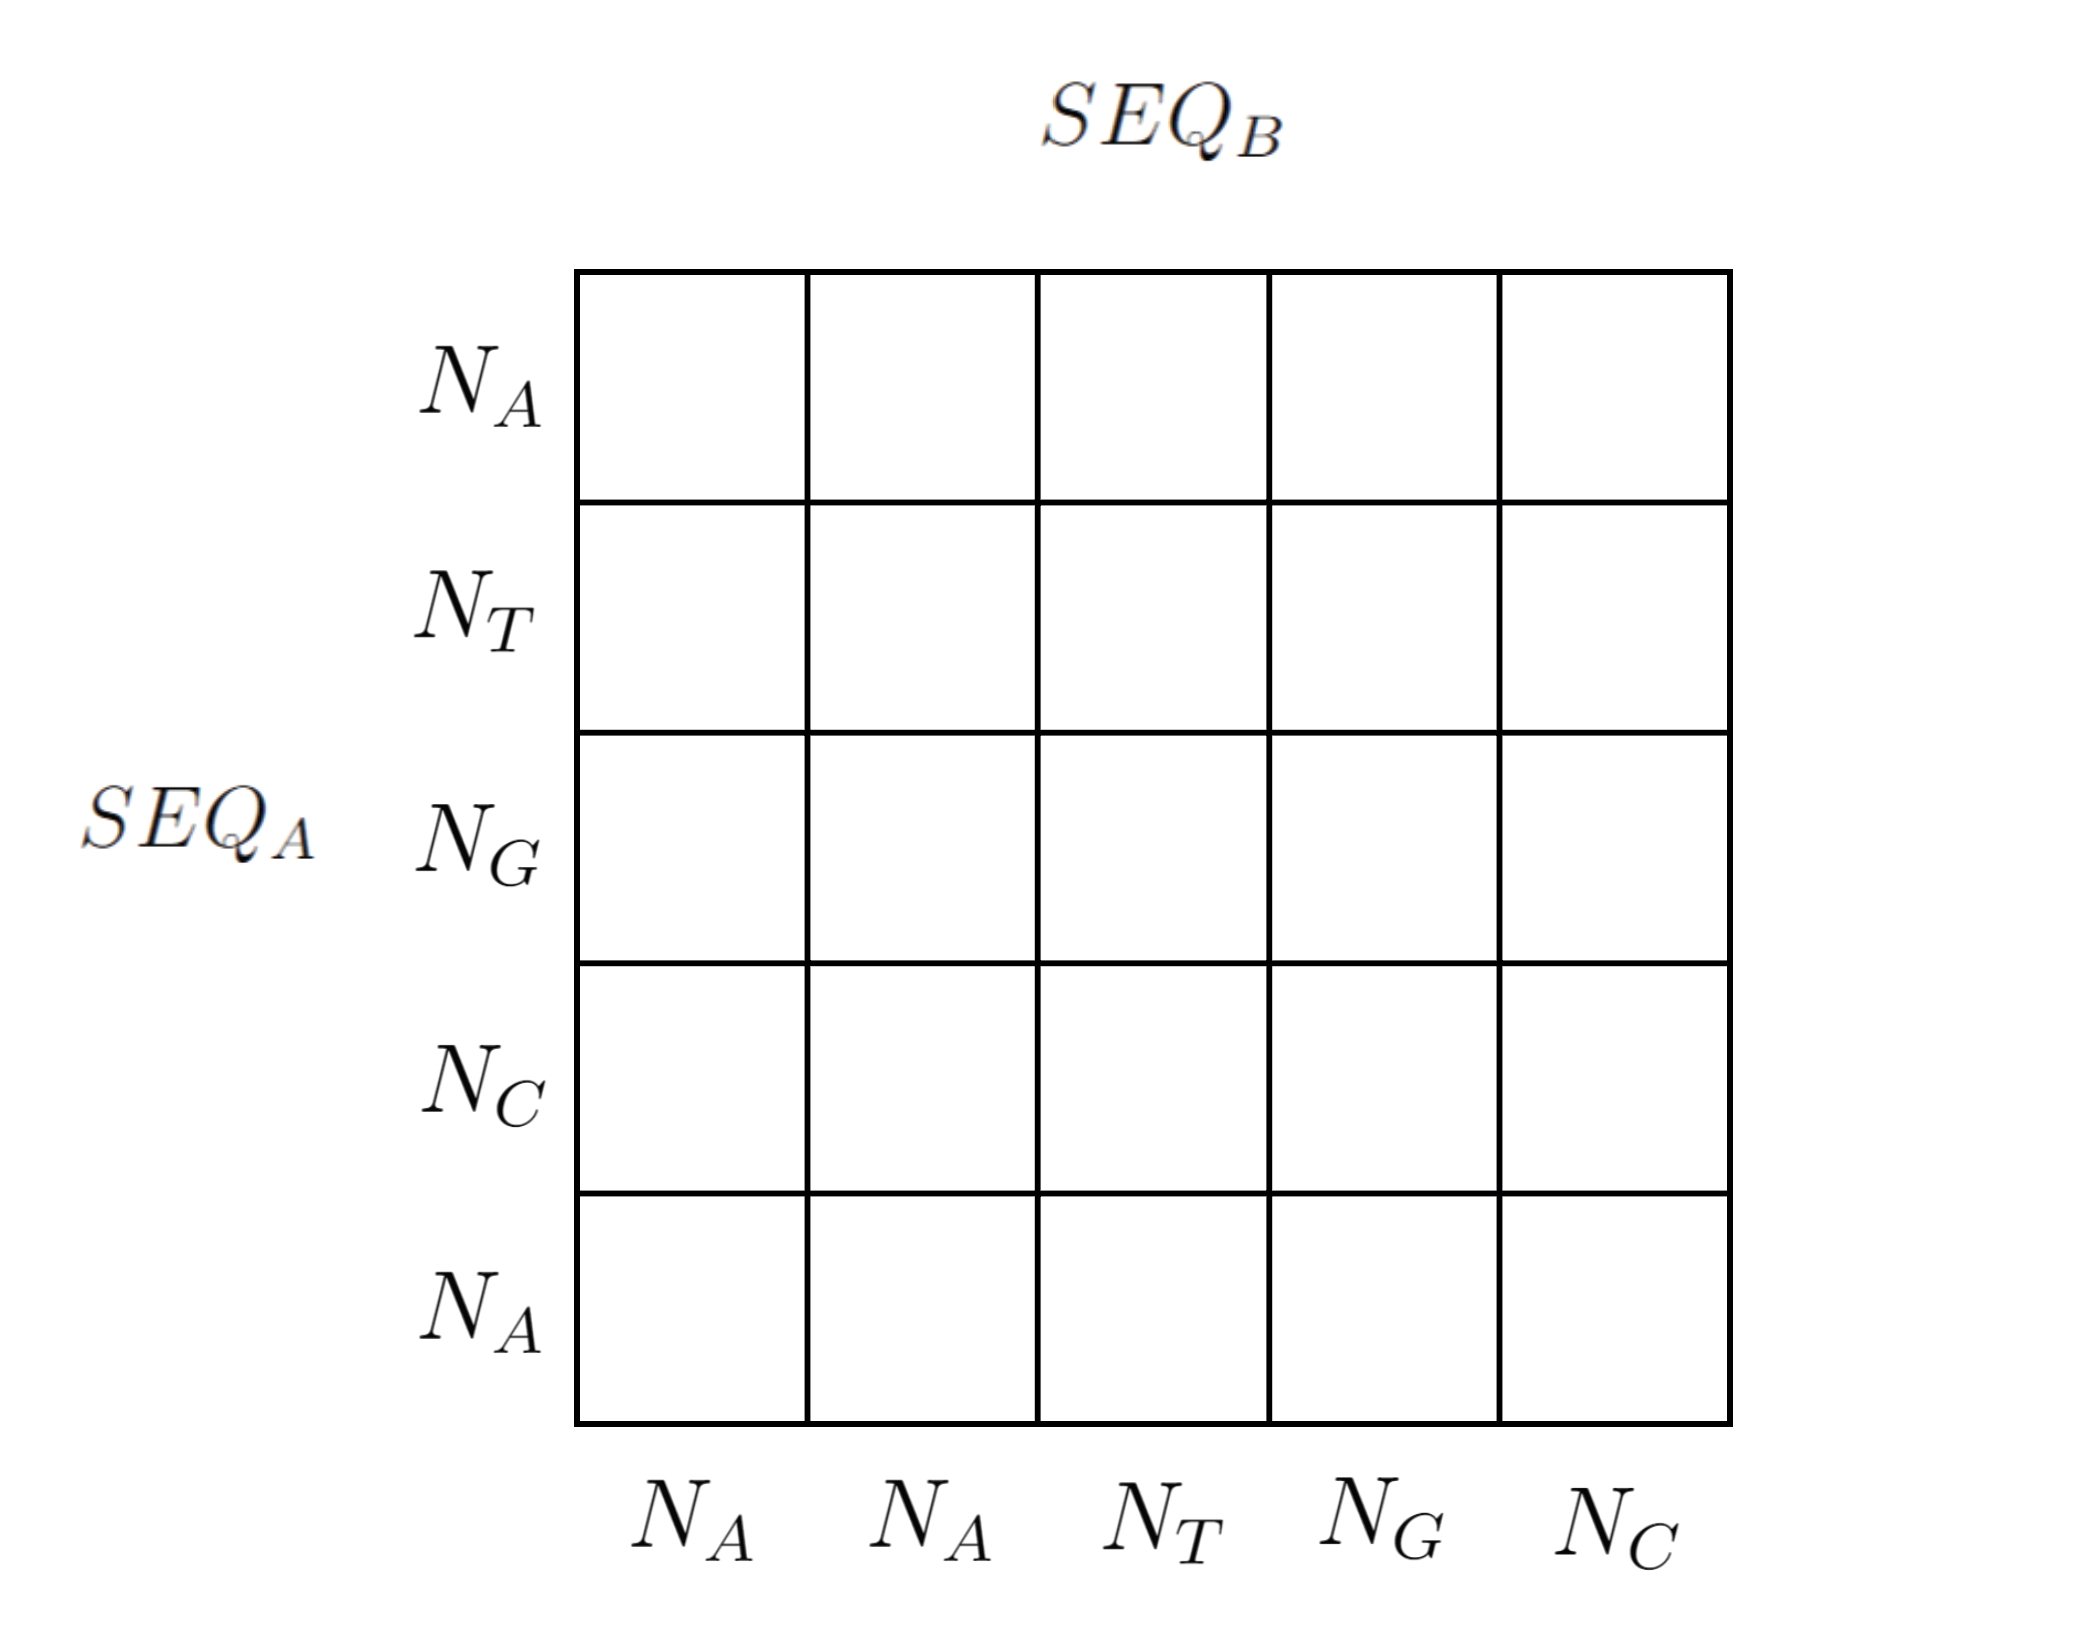
\includegraphics[width=0.5\textwidth]{physical_system_sublimat.png}
  }
  \caption{Pairwise comparison of genetic sequences}
  \label{fig:sequence_alignment}
  \end{center}
\end{figure}

\subsubsection{Goal Statements}


\noindent Given two genetic sequences of size n, the goal statements are:

\begin{itemize}

\item[GS\refstepcounter{goalnum}\thegoalnum \label{generate_alignment}:] Generate 
scores ranking the quality of the alignment between two genetic sequences given a 
benchmarked set of substitution matrices
% \item[GS\refstepcounter{goalnum}\thegoalnum \label{generate_rank}:] Rank  
% multiple substitution matrices by the quality of the alignments they produce

\end{itemize}

\subsection{Solution Characteristics Specification}

\begin{figure}[H]
  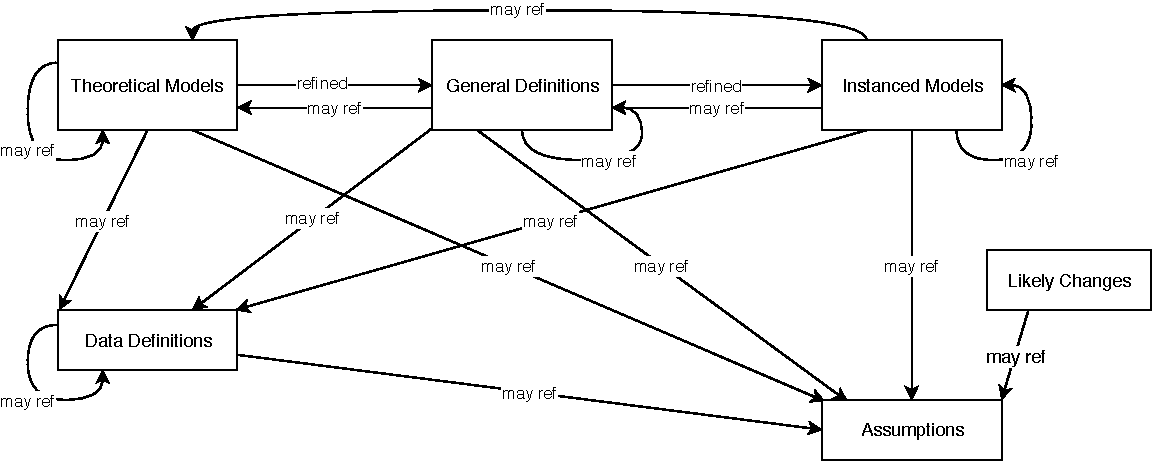
\includegraphics[scale=0.9]{RelationsBetweenTM_GD_IM_DD_A.pdf}
\end{figure}

The instance models that govern \progname{} are presented in
Subsection~\ref{sec_instance}.  The information to understand the meaning of the
instance models and their derivation is also presented, so that the instance
models can be verified.


\subsubsection{Assumptions} \label{sec_assumpt}


This section simplifies the original problem and helps in developing the
theoretical model by filling in the missing information for the physical system.
The numbers given in the square brackets refer to the theoretical model [TM],
general definition [GD], data definition [DD], instance model [IM], or likely
change [LC], in which the respective assumption is used.

\begin{itemize}

\item[A\refstepcounter{assumpnum}\theassumpnum \label{dna-sequences-only}:]
DNA-sequences-only: An alphabet of 4 letters, standardized to the genetic DNA nomenclature is used 
to represent the genetic sequences [DD\autoref{DD_substitution_matrices}]
\item[A\refstepcounter{assumpnum}\theassumpnum \label{two-sequences-only}:]
Two-sequences-only: The only valid number of genetic sequences to be compared is two [DD\autoref{DD_comparative_alginment_matrix}][GS\autoref{generate_alignment}][IM\autoref{IM_needleman_wunsch}].

\end{itemize}

\subsubsection{Theoretical Models}\label{sec_theoretical}



This section focuses on the general equations and laws that \progname{} is based
on.  
% \plt{Modify the examples below for your problem, and add additional models
%   as appropriate.}

~\newline

\noindent
\deftheory
% #2 refname of theory
{TM:DPO}
% #3 label
{Comparative alignment matrix}
% #4 equation
% {
%   % $F_{ij} = \max(F_{i-1,j-1} + S(SEQ_{A_i}, SEQ_{B_j}), F_{i,j-1} + g, F_{i-1,j} + g)$
%   $F_{i,j} = \max(F_{i-1,j-1} + S(A_{i}, B_{j}), F_{i,j-1} + d, F_{i-1,j} + d)$
% }
{
  % $F_{i,j} = \max(F_{i-1,j-1} + S(A_{i}, B_{j}), F_{i,j-1} + d, F_{i-1,j} + d)$
  $F_{ij} = \max(F_{i-1,j-1} + S(SEQ_{A_i}, SEQ_{B_j}), F_{i,j-1} + g, F_{i-1,j} + g)$
}
% #5 description
{
  % The above equation gives the optimal alignment score between two genetic sequences $A_{i}$ and $B$,
  % where $F_{i,j}$ is the alignment score at position $i$ in genetic sequence $A$ and position $j$ in 
  % genetic sequence $B$, $d$ is the gap penalty associated with a deletion or insertion, and $S$ is the substitution matrix.

  The above equation fills the values of the comparison matrix $F$ (a matrix of size $|SEQ_A| * |SEQ_B|$, with every $F_{i,j}$ in qa units)
  , where $F_{i,j}$ is a cell at $SEQ_A$ position $i$ (rows) and position $j$ in $SEQ_B$ 
   (columns); $g$ is the gap penalty associated with a deletion 
  or insertion (given in qa units); $ S \text{()} $ is a function that uses a substitution matrix to evaluate the
  nucleotide at position $SEQ_{A_i}$ and $SEQ_{B_j}$, returning a score given in qa units. The equation contains the 
  following edge cases: $F_{0,0} = 0$, $F_{i,0} = F_{i-1,0} + g$, and $F_{0,j} = F_{0,j-1} + g$.

  
  % F_{0,0} = 0 \\
  % F_{i,0} = F_{i-1,0} + g \\
  % F_{0,j} = F_{0,j-1} + g
  % The above equation gives the conservation of energy for transient heat transfer in a material
  % of specific heat capacity $C$ (\si{\joule\per\kilogram\per\celsius}) and density $\rho$ 
  % (\si{\kilogram\per\cubic\metre}), where $\bf q$ is the thermal flux vector (\si{\watt\per\square\metre}),
  % $g$ is the volumetric heat generation
  % (\si{\watt\per\cubic\metre}), $T$ is the temperature
  % (\si{\celsius}),  $t$ is time (\si{\second}), and $\nabla$ is
  % the gradient operator.  For this equation to apply, other forms
  % of energy, such as mechanical energy, are assumed to be negligible in the
  % system (\aref{A_OnlyThermalEnergy}).  In general, the material properties ($\rho$ and $C$) depend on temperature.
}
% #6 Notes
{
None.
}
% #7 Source
{
  \href{https://en.wikipedia.org/wiki/Needleman-Wunsch_algorithm}{Needleman-Wunsch Algorithm}, \cite{NEEDLEMAN1970443}
  % \url{https://en.wikipedia.org/wiki/Needleman-Wunsch_algorithm}
}
% #8 Referenced by
{
  % \dref{ROCT}
  --
}
% #9 Preconditions
{
None
}
% #1 derivation - not applicable by default
{}

~\newline

\subsubsection{General Definitions}\label{sec_gendef}


This section collects the laws and equations that will be used in building the
instance models.




\subsubsection{Data Definitions}\label{sec_datadef}



This section collects and defines all the data needed to build the instance
models. The dimension of each quantity is also given.  
% \plt{Modify the examples
%   below for your problem, and add additional definitions as appropriate.}

~\newline

% %%%%%%%%%%%%%%%%%%%%%%%%%%%%%%%%%%%%%%


% %%%%%%%%%%%%%%%%%%%%%%%%%%%%%%%%%%%%%%

\noindent
\begin{minipage}{\textwidth}
\renewcommand*{\arraystretch}{1.5}
\begin{tabular}{| p{\colAwidth} | p{\colBwidth}|}
\hline
\rowcolor[gray]{0.9}
Number& DD\refstepcounter{datadefnum}\thedatadefnum \label{DD_substitution_matrices}\\
\hline
Label& \bf Set of substitution matrices\\
\hline
Symbol &$\mathbb{S}$\\
\hline
% Units& $Mt^{-3}$\\
% \hline
  Units & -- \\
  \hline
  Equation&$S_k \in \{S_1, S_2, ..., S_n\}$\\
  \hline
  Description & 
                Set of substitution matrices that will be used
                to calculate the alignment quality between two genetic sequences.
                Each matrix $S_k$ is a square matrix of size 4x4, where each element
                belongs to one of the four letters of the genetic DNA nomenclature.
  \\
  \hline
  Sources& -- \\
  \hline
  Ref.\ By & \iref{IM_needleman_wunsch}\\
  \hline
\end{tabular}
\end{minipage}\\

% ##########################################################
\noindent
\begin{minipage}{\textwidth}
\renewcommand*{\arraystretch}{1.5}
\begin{tabular}{| p{\colAwidth} | p{\colBwidth}|}
\hline
\rowcolor[gray]{0.9}
Number& DD\refstepcounter{datadefnum}\thedatadefnum \label{DD_optimal_alignment_score}\\
\hline
Label& \bf Optimal alignment score\\
\hline
Symbol &$\text{Score}$\\
\hline
Units & qa \\
\hline
Equation&$\text{Score}(F, S_k) = \sum_{(i,j) \in \text{Path}} F_{i,j}$\\
\hline
Description & 
            The sum of alignment scores along the optimal path through
            matrix $F$. The optimal path is determined by tracing backwards
            from position $(m,n)$ to $(0,0)$, choosing at each step the
            direction that contributed to the current cell's value.
\\
\hline
Sources& -- \\
\hline
Ref.\ By & \iref{IM_needleman_wunsch}\\
\hline
\end{tabular}
\end{minipage}\\

% ##########################################################

\noindent
\begin{minipage}{\textwidth}
\renewcommand*{\arraystretch}{1.5}
\begin{tabular}{| p{\colAwidth} | p{\colBwidth}|}
\hline
\rowcolor[gray]{0.9}
Number& DD\refstepcounter{datadefnum}\thedatadefnum \label{DD_functionS}\\
\hline
Label& \bf Substitution matrix mapper\\
\hline
Symbol &$S(SEQ_{A_i}, SEQ_{B_j})$\\
\hline
Units & qa \\
\hline
Equation&$\text{Score}(F, S_k) = \sum_{(i,j) \in \text{Path}} F_{i,j}$\\
\hline
Description & 
            The sum of alignment scores along the optimal path through
            matrix $F$. The optimal path is determined by tracing backwards
            from position $(m,n)$ to $(0,0)$, choosing at each step the
            direction that contributed to the current cell's value.
\\
\hline
Sources& -- \\
\hline
Ref.\ By & \iref{IM_needleman_wunsch}\\
\hline
\end{tabular}
\end{minipage}\\




\subsubsection{Instance Models} \label{sec_instance}    

% \plt{The motivation for this section is to reduce the problem defined in
%   ``Physical System Description'' (Section~\ref{sec_phySystDescrip}) to one
%   expressed in mathematical terms. The IMs are built by refining the TMs and/or
%   GDs.  This section should remain abstract.  The SRS should specify the
%   requirements without considering the implementation.}

This section transforms the problem defined in Section~\ref{Sec_pd} into 
one which is expressed in mathematical terms. It uses concrete symbols defined 
in Section~\ref{sec_datadef} to replace the abstract symbols in the models 
identified in Sections~\ref{sec_theoretical} and~\ref{sec_gendef}.


% The goals \plt{reference your goals} are solved by \plt{reference your instance
%   models}.  

% \plt{other details, with cross-references where appropriate.}
% \plt{Modify the examples below for your problem, and add additional models as
%   appropriate.}

~\newline

%Instance Model 1
The goal \gsref{generate_alignment} is met by \iref{IM_needleman_wunsch}. 

\noindent
\begin{minipage}{\textwidth}
\renewcommand*{\arraystretch}{1.5}
\begin{tabular}{| p{\colAwidth} | p{\colBwidth}|}
  \hline
  \rowcolor[gray]{0.9}
  Number& IM\refstepcounter{instnum}\theinstnum \label{IM_needleman_wunsch}\\
  \hline
  Label& $O$\\
  \hline
  Input&$SEQ_A$,$SEQ_B$,$S_k$,$g$\\
  \hline
  Output&$O_{SEQ_{AB}}$\\
  \hline
  % Description& $O_{AB} = \forall S_k \in \mathbb{S} : F_{i,j}^k = \max(F_{i-1,j-1}^k + S_k(SEQ_A, SEQ_B), F_{i,j-1}^k + g, F_{i-1,j}^k + g)$\\
  % Description& $O_{AB} = \{F_{m,n}^{k=1}, \ldots, F_{m,n}^{ k=|S|}\} \quad \text{where} \quad m = |SEQ_A|, n = |SEQ_B|$\\
  Description & $O_{AB} = \{\text{Score}(F_{SEQ_A,SEQ_B}, S_k) \mid S_k \in \mathbb{S}\}$\\
  &Where\\
  & $SEQ_A$ and $SEQ_B$ are biological genetic sequences with bp units\\
  & $S_k$ is a substitution matrix element of $\mathbb{S}$\\
  & $g$ is the gap penalty given in qa units\\
  & $F$ is comparison matrix between sequences, with each cell given in qa units\\
  % &$\text{For each } S_k \in \mathbb{S}, \text{ matrix } F^k \text{ is computed as:}$\\
  % &$SEQ_A$ and $SEQ_B$ are biological genetic sequences with bp units\\
  % &$S_k$ is a substitution matrix element of $\mathbb{S}$\\
  % &$g$ is the gap penalty given in qa units\\
  % &$F$ is comparison matrix between sequences, with each cell given in qa units\\
  \hline
  Sources& -- \\
  \hline
  Ref.\ By & --\\
  \hline
\end{tabular}
\end{minipage}\\

%~\newline

% \subsubsection*{Derivation of ...}

% \plt{The derivation shows how the IM is derived from the TMs/GDs.  In cases
%   where the derivation cannot be described under the Description field, it will
%   be necessary to include this subsection.}

\subsubsection{Input Data Constraints} \label{sec_DataConstraints}    

Table~\ref{TblInputVar} shows the data constraints on the input output
variables.  The column for physical constraints gives the physical limitations
on the range of values that can be taken by the variable.  The column for
software constraints restricts the range of inputs to reasonable values.  The
software constraints will be helpful in the design stage for picking suitable
algorithms.  The constraints are conservative, to give the user of the model the
flexibility to experiment with unusual situations.  The column of typical values
is intended to provide a feel for a common scenario.  The uncertainty column
provides an estimate of the confidence with which the physical quantities can be
measured.  This information would be part of the input if one were performing an
uncertainty quantification exercise.

% The specification parameters in Table~\ref{TblInputVar} are listed in
% Table~\ref{TblSpecParams}.

\begin{table}[!h]
  \caption{Input Variables} \label{TblInputVar}
  \renewcommand{\arraystretch}{1.2}
\noindent \begin{longtable*}{l l l l c} 
  \toprule
  \textbf{Var} & \textbf{Physical Constraints} & \textbf{Software Constraints} &
                             \textbf{Typical Value} & \textbf{Uncertainty}\\
  \midrule 
  $SEQ_A$ & $|{seq_A}| \geq 1$ & $|seq_A| \approx |seq_B|$ & 1 kb & 40\%
  \\
  $SEQ_B$ & $|{seq_B}| \geq 1$ & $|seq_B| \approx |seq_A|$ & 1 kb & 40\%
  \\
  $S_k$ & $S \in \mathbb{R}^{n \times n}, n \geq 4$ & $S \in \mathbb{R}^{n \times n}, n \geq 0$ & $S \in \mathbb{R}^{4 \times 4}$& 0\%
  \\
  $F$ & $F \in \sum|seq_i| \times |seq_j|$ & $|seq_i|, |seq_j| \geq 1$ & $\approx 1 kb^2$ & 20\%
  \\
  $g$ & $g \in \mathbb{R}_{\leq 0}$ & -- & $-2$ & 10\%
  \\
  $O_{AB}$ & $O_{AB} \in \mathbb{R}^{m \times n}, m,n \geq 1$ & -- & *$\vec{v} = [0,-2,-12]$ & 0\%
  \\
  \bottomrule
\end{longtable*}
\end{table}

\noindent 



\section{Requirements}

% \plt{The requirements refine the goal statement.  They will make heavy use of
%   references to the instance models.}

This section provides the functional requirements, the business tasks that the
software is expected to complete, and the nonfunctional requirements, the
qualities that the software is expected to exhibit.

\subsection{Functional Requirements}

\noindent \begin{itemize}

\item[R\refstepcounter{reqnum}\thereqnum \label{R_Inputs}:] Input $SEQ_A$, $SEQ_B$ as 
strings of base pair units (bp), substitution matrix $S \in \mathbb{R}^{n \times n}$, and gap penalty $g \in \mathbb{R}_{<0}$.

% \plt{Requirements
%     for the inputs that are supplied by the user.  This information has to be
%     explicit.}

\item[R\refstepcounter{reqnum}\thereqnum \label{R_OutputInputs}:] Use the inputs 
stated in \iref{R_Inputs} to build a comparative matrix $F^k$ for 
each substitution matrix $S_k$ in $\mathbb{S}$.

% \plt{It isn't
%   always required, but often echoing the inputs as part of the output is a
%   good idea.}

\item[R\refstepcounter{reqnum}\thereqnum \label{R_Calculate}:] Calculate optimal 
alignment scores \iref{IM_needleman_wunsch}.

\item[R\refstepcounter{reqnum}\thereqnum \label{R_VerifyOutput}:] Verify that:
\begin{itemize}
\item Input sequences contain only valid nucleotides (A,T,C,G)
\item Sequences meet minimum length requirement $|seq_i|, |seq_j| \geq 1$
\item Gap penalty is negative $g < 0$
\item Substitution matrices are square $n \times n$
\end{itemize}

\item[R\refstepcounter{reqnum}\thereqnum \label{R_Output}:] Output:
\begin{itemize}
\item Aligned sequences with gap insertions
\item Alignment scores for each $S_k$
\item Ranking of substitution matrices by alignment quality
\end{itemize}

\end{itemize}

% \plt{Every IM should map to at least one requirement, but not every requirement
%   has to map to a corresponding IM.}

\subsection{Nonfunctional Requirements}


\noindent \begin{itemize}

  \item[NFR\refstepcounter{nfrnum}\thenfrnum \label{NFR_Accuracy}:]
  \textbf{Accuracy} The alignment quality scores produced by \progname{} shall meet the 
  precision requirements needed for comparative biology research. 
  
  \item[NFR\refstepcounter{nfrnum}\thenfrnum \label{NFR_Usability}:] \textbf{Usability}
  Users with knowledge of genetics and comparative biology, as described in Section~\ref{SecUserCharacteristics}, 
  should be able to successfully use the software with minimal training. 
  The interface shall accept standard sequence formats and provide clear visualization of alignments.
  
  \item[NFR\refstepcounter{nfrnum}\thenfrnum \label{NFR_Maintainability}:]
  \textbf{Maintainability} The effort required to modify or extend \progname{} 
  with new substitution matrices (e.g. protein matrices) should be less than 5\% 
  of the original development time, and no more than 40\% of the original development time 
  for new alignment algorithms (e.g. heuristics).
  
  \item[NFR\refstepcounter{nfrnum}\thenfrnum \label{NFR_Portability}:]
  \textbf{Portability} \progname{} shall run on Linux, Windows 10+, and MacOS 13+ operating systems.
  
  \item[NFR\refstepcounter{nfrnum}\thenfrnum \label{NFR_Performance}:]
  \textbf{Performance} \progname{} shall complete alignment calculations for sequences of length n in O(n²) time complexity.

\end{itemize}

\subsection{Rationale}

The rationale behind the assumption \aref{dna-sequences-only} relies on the unique 
benchmarking properties of the set $\mathbb{S}$ that contains only DNA substitution matrices.
This improves on the user experience and improves the modularity in the software, enhancing 
maintainability and portability, which are key nonfunctional requirements.

The second rationale that justifies assumption \aref{two-sequences-only} is the
nature of the Needleman-Wunsch algorithm, which guarantees optimal alignment in 2D matrices.

\section{Likely Changes}    

\noindent \begin{itemize}

\item[LC\refstepcounter{lcnum}\thelcnum\label{LC_expand_matrices}:]
The software may be extended to include protein sequences, which will require
expanding the set of substitution matrices $\mathbb{S}$ to include protein matrices.

\end{itemize}

\section{Unlikely Changes}    

\noindent \begin{itemize}

\item[LC\refstepcounter{lcnum}\thelcnum\label{LC_keep_optimization_global}:] 
The dimensionality of matrix $F$ shall remain 2D, as the Needleman-Wunsch algorithm
is designed to optimize global alignment scores.

\end{itemize}

\section{Traceability Matrices and Graphs}

The purpose of the traceability matrices is to provide easy references on what
has to be additionally modified if a certain component is changed.  Every time a
component is changed, the items in the column of that component that are marked
with an ``X'' may have to be modified as well.  Table~\ref{Table:trace} shows the
dependencies of theoretical models, general definitions, data definitions, and
instance models with each other. Table~\ref{Table:R_trace} shows the
dependencies of instance models, requirements, and data constraints on each
other. Table~\ref{Table:A_trace} shows the dependencies of theoretical models,
general definitions, data definitions, instance models, and likely changes on
the assumptions.


\begin{table}[h!]
\centering

\begin{tabular}{|c|c|c|c|c|c|}
\hline
  & \aref{dna-sequences-only}& \aref{two-sequences-only}& \tref{TM:DPO}& \ddref{DD_comparative_alginment_matrix}& \iref{IM_needleman_wunsch}\\
\hline
\aref{dna-sequences-only} & --&  &  &  &  \\ \hline
\aref{two-sequences-only} &  & --&  &  &  \\ \hline
\tref{TM:DPO} & X & X & --&  &  \\ \hline
\ddref{DD_comparative_alginment_matrix} & X & X &  & --&  \\ \hline
\iref{IM_needleman_wunsch} & X & X & X &  & --\\
\hline
\end{tabular}


\caption{Traceability Matrix Showing the Connections Between Assumptions and Other Items}
\label{Table:A_trace}
\end{table}
% \end{landscape}
% }

%%%%%%%%%%%%%%%%%%%%%%%%%%%%%%%%%%%%%

\begin{table}[h!]
\centering
\begin{tabular}{|c|c|c|c|c|}
\hline        
  & \tref{TM:DPO} & \ddref{DD_comparative_alginment_matrix} & \ddref{DD_substitution_matrices} & \iref{IM_needleman_wunsch} \\ \hline
\tref{TM:DPO} & -- & X &   & X \\ \hline
\ddref{DD_comparative_alginment_matrix} &   & -- &   &   \\ \hline
\ddref{DD_substitution_matrices} &   &   & -- &   \\ \hline
\iref{IM_needleman_wunsch} & X & X &   & -- \\ \hline
\end{tabular}
\caption{Traceability Matrix Showing the Connections Between Items of Different Sections}
\label{Table:trace}
\end{table}


\begin{table}[h!]
\centering
\begin{tabular}{|c|c|c|c|c|c|c|}
\hline
  & \iref{IM_needleman_wunsch} & \rref{R_Inputs} & \rref{R_OutputInputs} & \rref{R_Calculate} & \rref{R_VerifyOutput} & \rref{R_Output} \\ \hline
\iref{IM_needleman_wunsch} & -- & X & & X & & X \\ \hline
\rref{R_Inputs} & X & -- & X & & & \\ \hline
\rref{R_OutputInputs} & & X & -- & & & \\ \hline
\rref{R_Calculate} & X & & & -- & & X \\ \hline
\rref{R_VerifyOutput} & & X & & X & -- & \\ \hline
\rref{R_Output} & X & & & X & & -- \\ \hline
\end{tabular}
\caption{Traceability Matrix Showing the Connections Between Requirements and Instance Models}
\label{Table:R_trace}
\end{table}

The purpose of the traceability graphs is also to provide easy references on
what has to be additionally modified if a certain component is changed.  The
arrows in the graphs represent dependencies. The component at the tail of an
arrow is depended on by the component at the head of that arrow. Therefore, if a
component is changed, the components that it points to should also be
changed. Figure~\ref{Fig_ATrace} shows the dependencies of theoretical models,
general definitions, data definitions, instance models, likely changes, and
assumptions on each other. Figure~\ref{Fig_RTrace} shows the dependencies of
instance models, requirements, and data constraints on each other.

\begin{figure}[h!]
	\begin{center}
		%\rotatebox{-90}
		{
			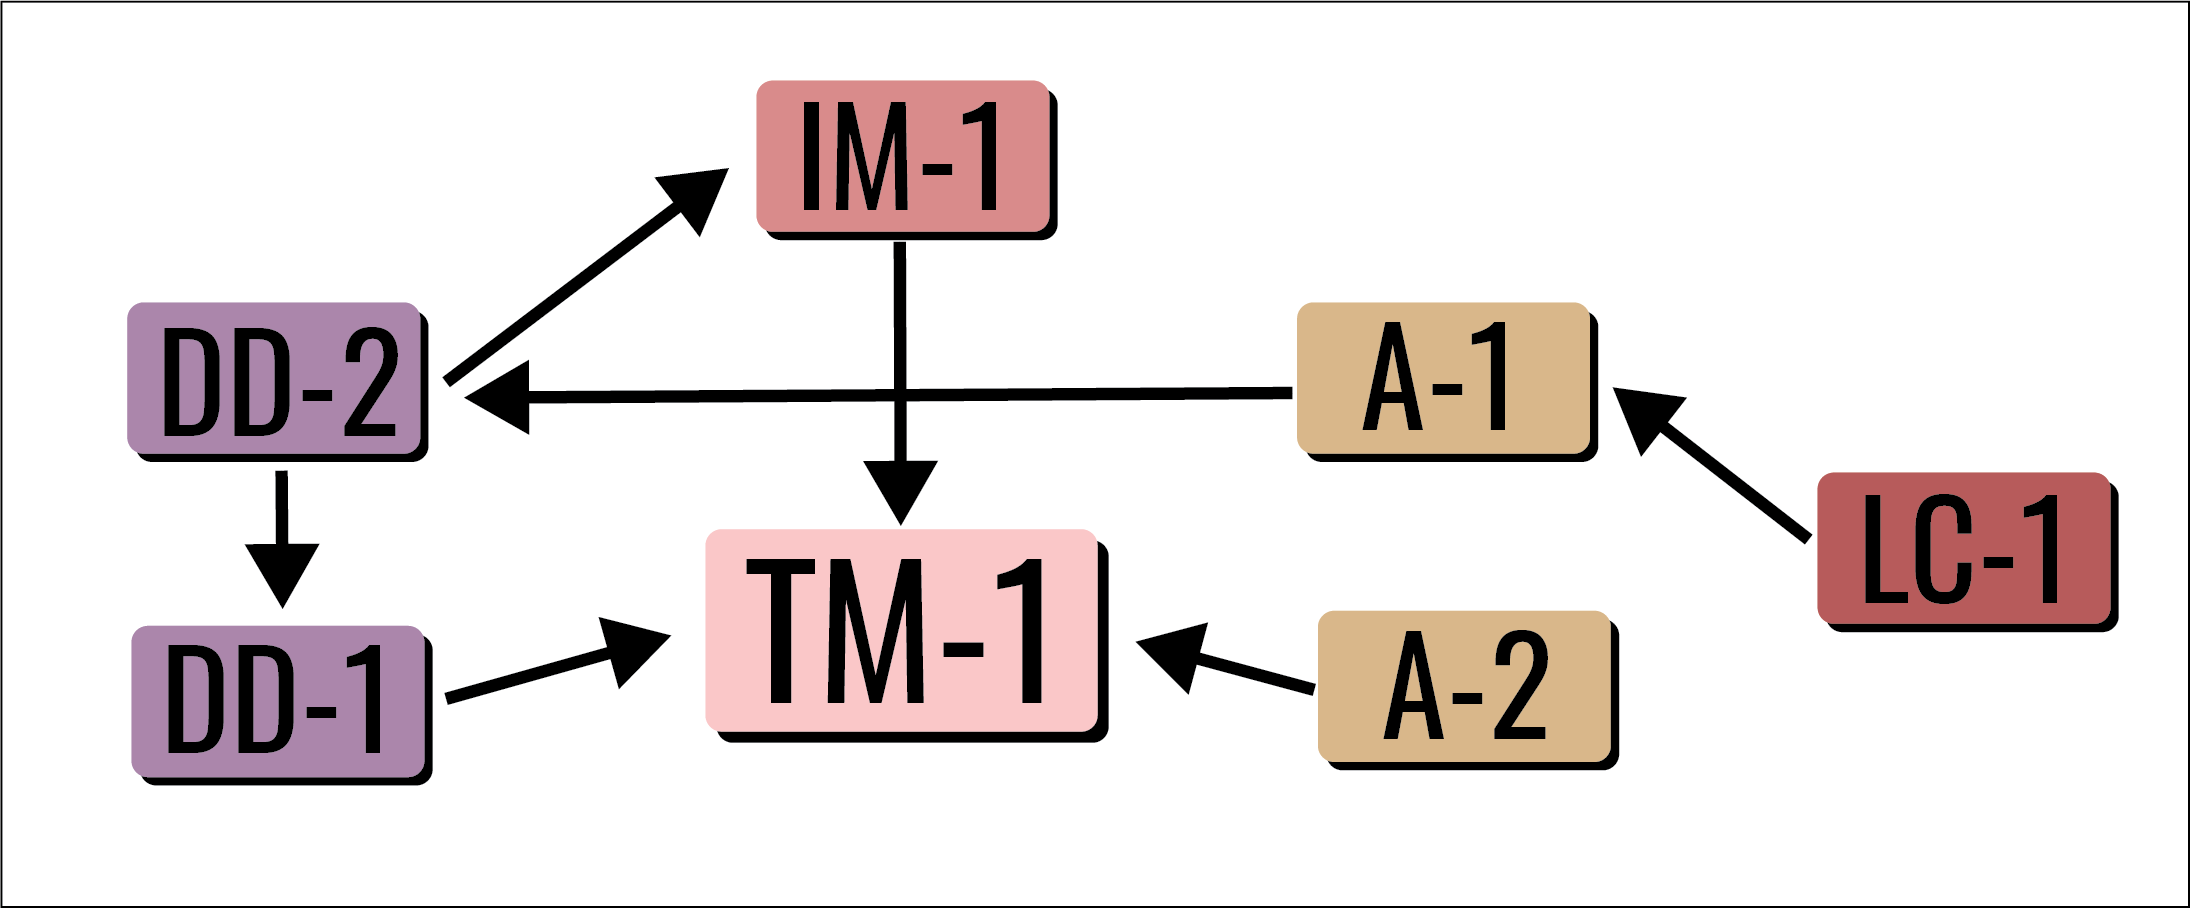
\includegraphics[width=\textwidth]{sublimat_atrace.png}
		}
		\caption{\label{Fig_ATrace} Traceability Matrix Showing the Connections Between Items of Different Sections}
	\end{center}
\end{figure}


\begin{figure}[h!]
	\begin{center}
		%\rotatebox{-90}
		{
			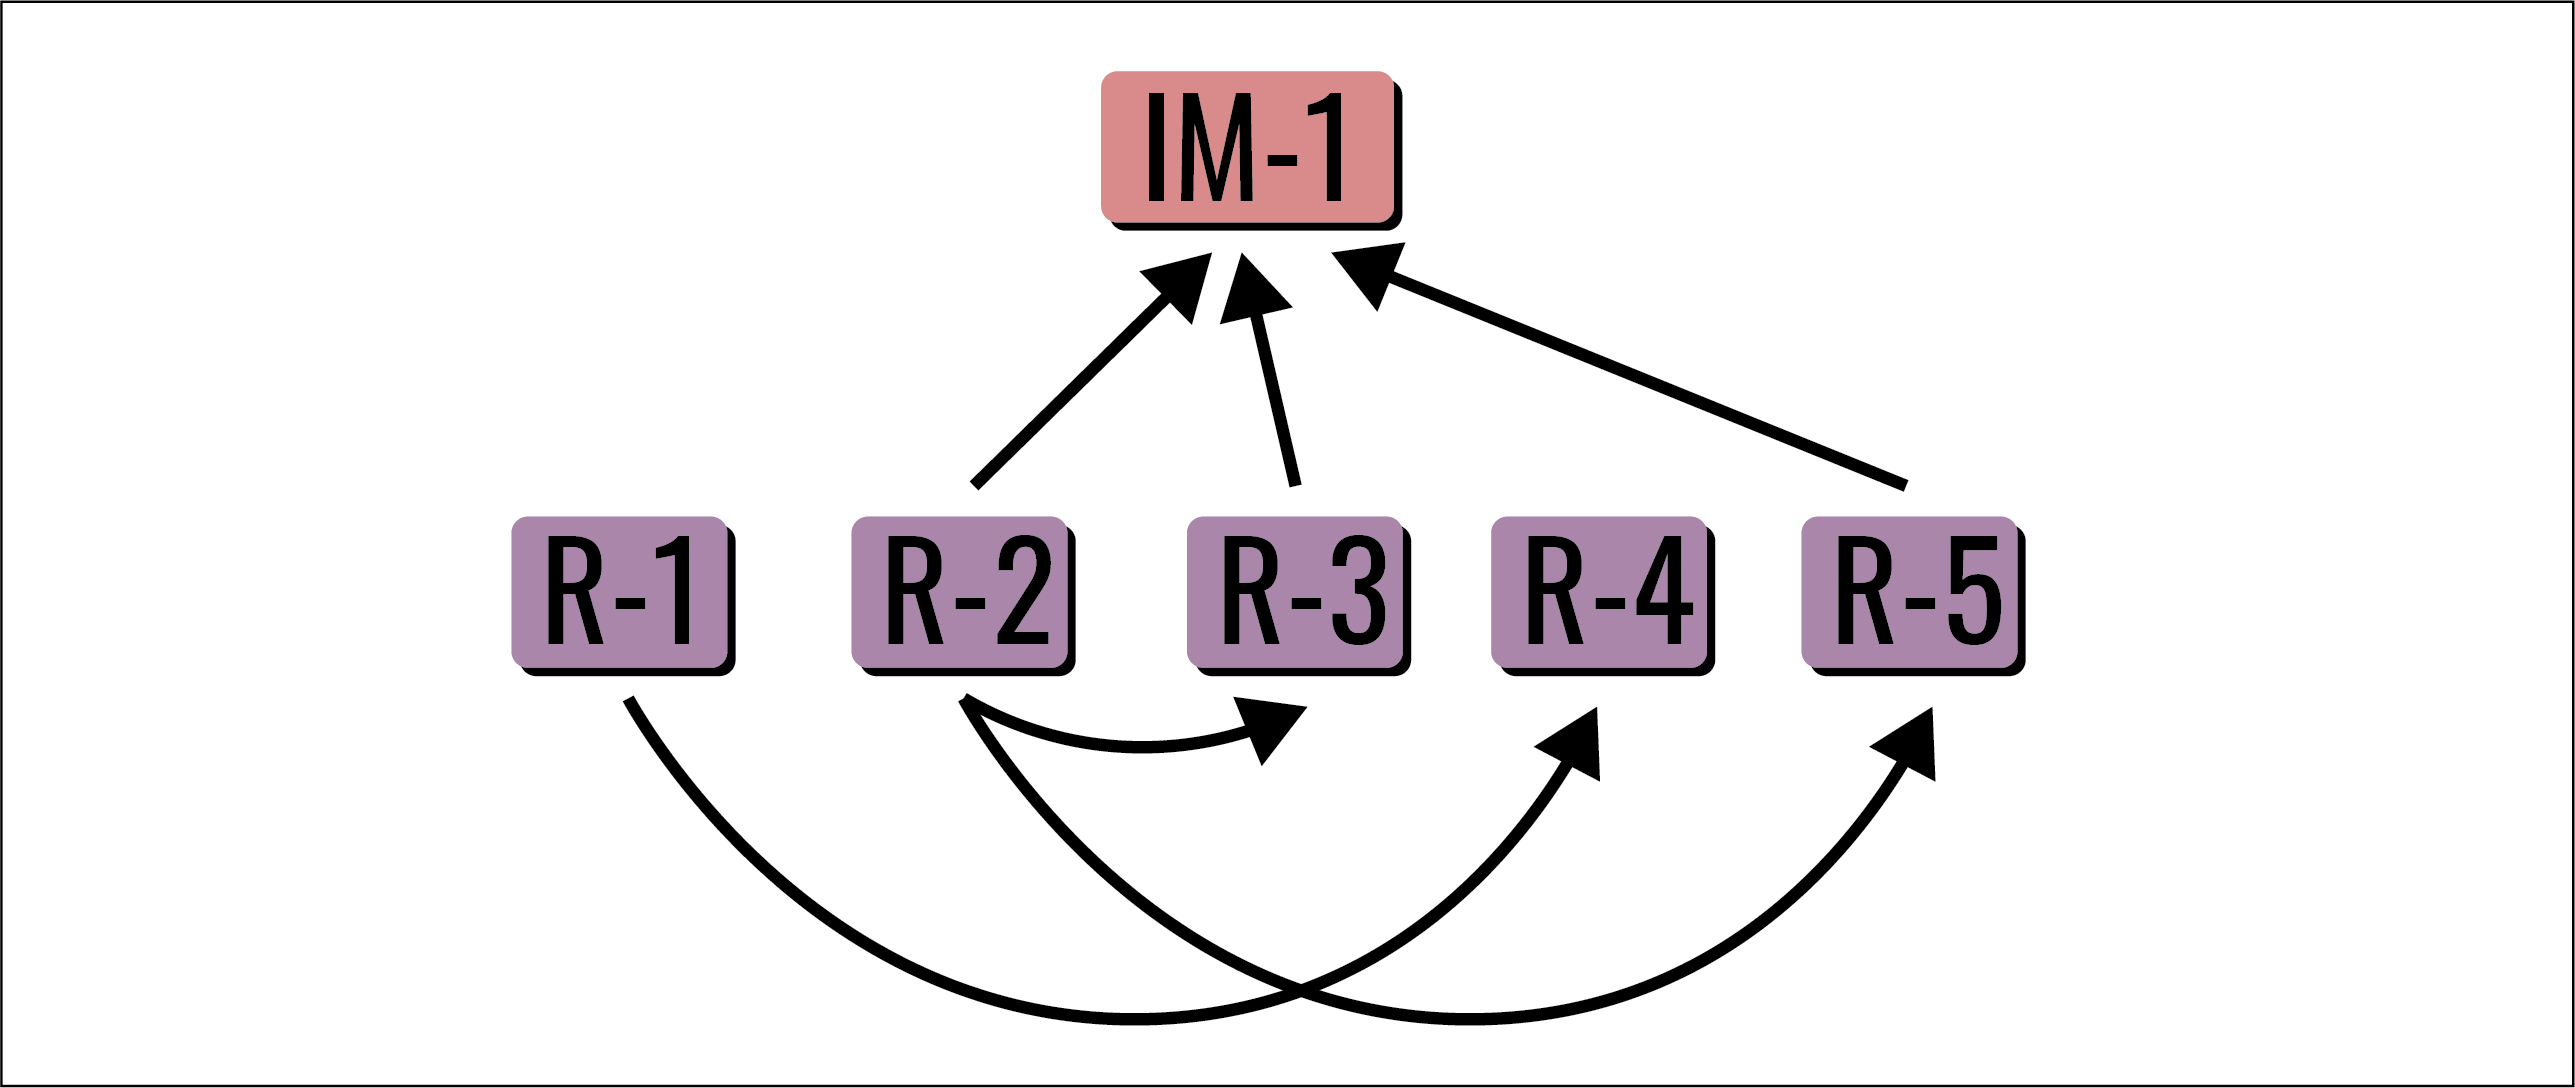
\includegraphics[width=0.7\textwidth]{sublimat_rtrace.png}
		}
		\caption{\label{Fig_RTrace} Traceability Matrix Showing the Connections Between Requirements, Instance Models, and Data Constraints}
	\end{center}
\end{figure}


\section{Values of Auxiliary Constants}

\newpage

\bibliographystyle {plainnat}
\bibliography {../../refs/References}

\end{document}